\section{Realios mašinos projektas}

\subsection{Techninės įrangos komponentai}

\begin{description}
\item[Procesorius] gali dirbti dviem režimais – supervizoriaus arba vartotojo. Naudotojo rėžime vykdomos virtualios mašinos komandos, o supervizoriaus rėžime – operacinės sistemos. Laiko tarpas, kurį procesorius atlieka vieną komandą laikomas vienu laiko vienetu. Procesorius turi šiuos registrus:
    \begin{description}
        \item[$IC$] - 2 baitų nuorodos registras. Skirtas nurodyti vykdomos virtualios mašinos komandos adresą atmintyje.
        \item[$R1$] - 4 baitų bendro naudojimo registras.
        \item[$R2$] - 4 baitų bendro naudojimo registras.
        \item[$SF$] - 2 baitų loginis registras, saugomi aritmetinių ir loginių operacijų suformuoti požymiai.
        \item[$MODE$] - 1 baito loginis registras, kurio reikšmė nusako procesoriaus darbo rėžimą („N“ – naudotojas, „S“ – supervizorius).
        \item[$PLR$] - 2 baitų registras nurodyti puslapių lentelės bloko adresą.
        \item[$PLBR$] - 2 baitų registras skirtas nurodyti puslapių lentelės pirmojo baito vietą PLR bloke.
        \item[$PI$] - 1 baito registras programiniams petraukiamams fiksuoti.
        \item[$SI$] - 1 baito registras supervizoriniams pertraukimams fiksuoti.
        \item[$TI$] - 1 baito taimerio registras.
        \item[$IOI$] - 1 baito įvedimo ir išvedimo petraukimų registras.
        \item[$CHST$] - 1 baito kanalų užimtumo registras.
    \end{description}
\end{description}

\begin{tabularx}{0.85\textwidth}{|c|c|c|X|} 
          \hline
          Bitas & Trumpinys & Reikšmė & Paaiškinimas \\
          \hline
          0 & CF & pernešimo požymis & įgija „1“ tada, kai sudėties arba
          atimties rezultatas netelpa į žodį \\
          \hline
          1 & ZF & nulio požymis & parodo ar paskutinės operacijos 
          rezultatas yra nulinis \\
          \hline
          2 & SF & ženklo požymis & parodo, koks yra paskutinės operacijos 
          rezultato ženklas („1“ – jei neigiamas) \\
          \hline
          11 & OF & perpildymo požymis & įgija „1“ tada, kai rezultatas
          netelpa skaičių su ženklu diapazone \\
          \hline
        \end{tabularx}

\begin{description}
\item[Atmintis] Atmintis – įrenginys informacijai saugoti. Mūsų reali mašina turi trijų rūšių atmintis: supervizorinę, skirtą OS poreikiams, vartotojo, virtualioms mašinoms, ir išorinę:
    \begin{description}
        \item[Supervizorinė] - jos dydis 16 blokų.
        \item[Vartotojo] - atmintis skirta virtualių mašinų atmintims bei puslapių lentelėms laikyti. Mes apibrėšime vartotojo atmintį taip: lentelės dydis – 2560 žodžių po 4 baitus. 160 žodžių laikysime bloku (takeliu). Taigi vartotojo atmintis lygi 160-kai blokų, sunumeruotų nuo 0 iki 15, arba 2560 žodžių, sunumeruotų nuo 0 iki 2565.
        \item[Išorinė] - bus realizuota failu - kietuoju disku. Tarkime laikysime kad faile yra 1600 blokų. Išorinę atmintį galima pavaizduoti analogiškai vartotojo atminčiai, tik ji nėra dalijama į kitas atmintis. Failo pradžioje aprašoma kietojo disko struktūra su jame esančiais failais, jų pradžios blokais ir ilgiais.
    \end{description}
\end{description}

\begin{description}
\item[Taimeris] - Šis mechanizmas atsakingas už geresnį užduočių išlygiagretinimą. Yra laikoma kad ta pati užduotis negali būti vykdoma ilgiau nei N laiko momentų. Bus vykdoma ne daugiau N einamosios užduoties taktų. Laikysim, kad visos instrukcijos atliekamos per 1 taktą. Pradedant virtualios mašinos užduoties vykdymą TI registro reikšmė nustatoma tam tikrai reikšmei. Tarkim N = 10. Įvykdžius eilinę instrukciją TI reikšmė mažinama priklausomai nuo to per kiek taktų ši instrukcija yra atliekama. Kuomet TI reikšmė yra lygi nuliui, mikrokomanda Test () aptinka taimerio pertraukimą.
\end{description}

\begin{description}
\item[Pertraukimai] - tai signalas apie įvykusį įvykį. Kiekvienas pertraukimas turi savo
identifikaciją. Pertraukimą sistema turi aptikti ir atitinkamai sureaguoti. Kompiuterio būseną keičia tą būseną sukėlusi priežastis, pavyzdžiui, jei virtuali mašina vykdydama vartotojo programą sutinka neteisingą adresą ar operacijos kodą, tai komandų interpretatorius fiksuoja požymį “neteisingas adresas” (priskiria pertraukimo registrui tam tikrą reikšmę). Pertraukimus aptinka procesoriaus komanda test, kuri apklausia reikalingus registrus. Ir tik sistemai aptikus pertraukimą, yra nutraukiamas vartotojo programos vykdymas. Tai atliekama pasinaudojant pertraukimų vektorių lentele (kur yra nuorodos į pertraukimus apdorojančias programas). Valdymas yra perduodamas pertraukimą
apdorosiančiai programai, kuri dažniausiai yra atmintyje su požymiu “tik skaitymui”. Įvykdžiusi savo darbą, pertraukimo apdorojimo programa valdymą gražina operacinei sistemai pertraukimo vietoje. Bus realizuoti trijų tipų pertraukimai – programiniai, supervizoriniai ir taimerio. Programinių pertraukimų registras yra PI, supervizorinių pertraukimų registras – SI, taimerio - TI. Programiniai pertraukimai kyla vykdant virtualią mašiną, bandant įvykdyti kokį nors neleistiną veiksmą arba nuskaičius neleistiną reikšmę. Supervizoriniai pertraukimai kyla virtualiai mašinai norint įvykdyti veiksmą, kuris gali vykti tik supervizoriaus režime. Pertraukimai gali būti aptikti tik vartotojo režime. Supervizoriniame režime centrinio procesoriaus darbo pertraukti negalima. Pertraukimai kils šiais būdais:
    \begin{description}
    \item Operacijos GD, PD ir HALT iššauks supervizorinius pertraukimus. SI = 1 - komanda GD, SI = 2 - komanda PD, SI = 3 – komanda HALT.
    \item Programiniai pertraukimai: PI = 1 – neteisingas adresas, PI = 2 – neteisingas operacijos kodas, PI = 3 – neteisingas priskyrimas, PI = 4 – perpildymas (overflow).
    \item Esant TI = 0 bus fiksuojamas taimerio pertraukimas.
    \end{description}
Esant situacijai SI = 0 ir PI = 0 ir TI <> 0, pertraukimų sistema neaptiks. Pertraukimai nustatomi paprasčiausiai virtualaus procesoriaus registrams priskiriant atitinkamas reikšmes (pavyzdžiui, komandų interpretatoriui vykdant komandą GD, jis priskiria SI:= 1) Kiekvieną kartą komandų interpretatoriui įvykdžius programą, kviečiama komanda test(), kuri apklausia registrus, ir, jei kilo pertraukimas, gražina informaciją apie tai. Komanda test() gali būti tokia:
\begin{verbatim}
    If ((PI + SI) > 0) or (TI = 0) then return 1 else return 0;
\end{verbatim}
Nustačius įvykusį pertraukimą (t.y. test() <> 0) virtualios mašinos procesoriaus registrų reikšmės yra išsaugomos, procesorius perjungiamas į supervizoriaus režimą, nustatomas pertraukimo pobūdis (pavyzdžiui tiesiogiai apklausiant registrus) ir kviečiama pertraukimą apdorosianti paprogramė. Vėliau valdymas grįžta į virtualią mašiną, registrai atstatomi, procesorius perjungiamas į vartotojo režimą, ir operacinė sistema sprendžia, ką daryti toliau.
\end{description}



\item{Įvedimo įrenginiai}

\begin{figure}[H]
        \centering
        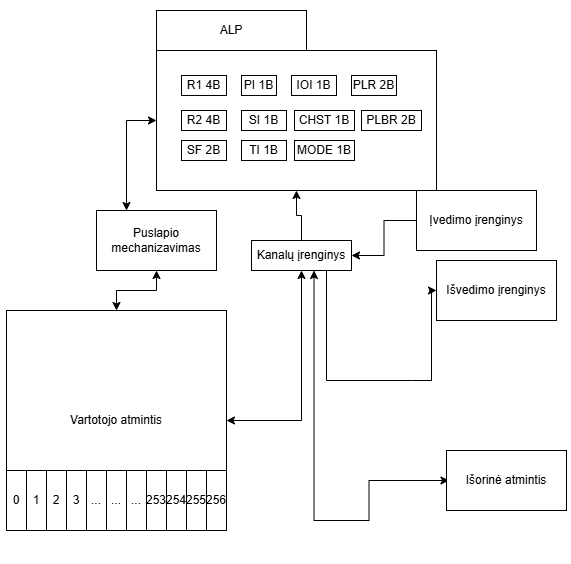
\includegraphics[width=1\linewidth]{reali masina.png}
        \caption{Reali masina}
        \label{fig:placeholder}
    \end{figure}
